%! Date = 4/23/25
\section{Motivation}\label{sec:motivation}
\begin{table}[!ht]
    \centering
    \caption{Straggler Delay within Synchronous \emph{All-to-All} communication.
    We capture the distribution of delay induced by stragglers across many steps.
    Let \textbf{Actual Time} $t_a$ denote the fastest kernel execution time across all GPUs,
        and \textbf{Total Time} $t$ be the maximum recorded step time. We define
        $Delay$ as the maximum difference between $t$ and $t_a$. Note $Delay$ is idle time. For the
        1x8 V100, we profile 1750 steps and 600 steps for the 8x4 A100. See Figure~\ref{fig:straggler}
        for the raw disribution.}
    \label{tab:s_delays}
    \begin{tabular}{@{}lcccc@{}}
        \toprule
        \textbf{System}      & \multicolumn{1}{l}{\textbf{\# Nodes}} & \multicolumn{1}{l}{\textbf{\# GPUs}} & \textbf{Median} & \textbf{p95} \\ \midrule
        Commercial VM (V100) & 1                                     & 8                                    & 3.1x            & 11.4x        \\
        Supercomputer (A100) & 8                                     & 32                                   & 1.09x           & 1.32x        \\ \bottomrule
    \end{tabular}
\end{table}
\begin{table}[!h]
    \centering
    \caption{\textbf{Kernel Fusion Comparison.}
    Our method is the first to fully fuse the DMoE layer into a single GPU kernel. We report GPU operations from detailed profiling with Nsight Systems (\S\ref{sec:evaluation}).}
    \label{tab:gpuOps}
    \setlength{\tabcolsep}{8pt}
    \renewcommand{\arraystretch}{0.9}
    \begin{tabular}{@{}lc@{}}
        \toprule
        \textbf{Works} & \textbf{Launched GPU Ops} \\ \midrule
        \sysname & 1 \\
        COMET~\cite{comet} & 33 \\
        Megatron-LM CUTLASS~\cite{megatron, 10.1145/3458817.3476209} & 85 \\
        Megatron-LM TE~\cite{megatron, 10.1145/3458817.3476209} & 261 \\
        Megatron-LM + DeepEP~\cite{deepep} & 432 \\
        DeepSpeedMoE~\cite{pmlr-v162-rajbhandari22a} & 550 \\
        \bottomrule
    \end{tabular}
    \vspace{-0.4cm}
\end{table}
%~\cite{megascale,antdt,malleus,optireduce,sms}
\subsection{Synchronous Communication and Stragglers}\label{sec:synchronous-communication-and-stragglers}
\begin{figure}[!ht]
    \centering
    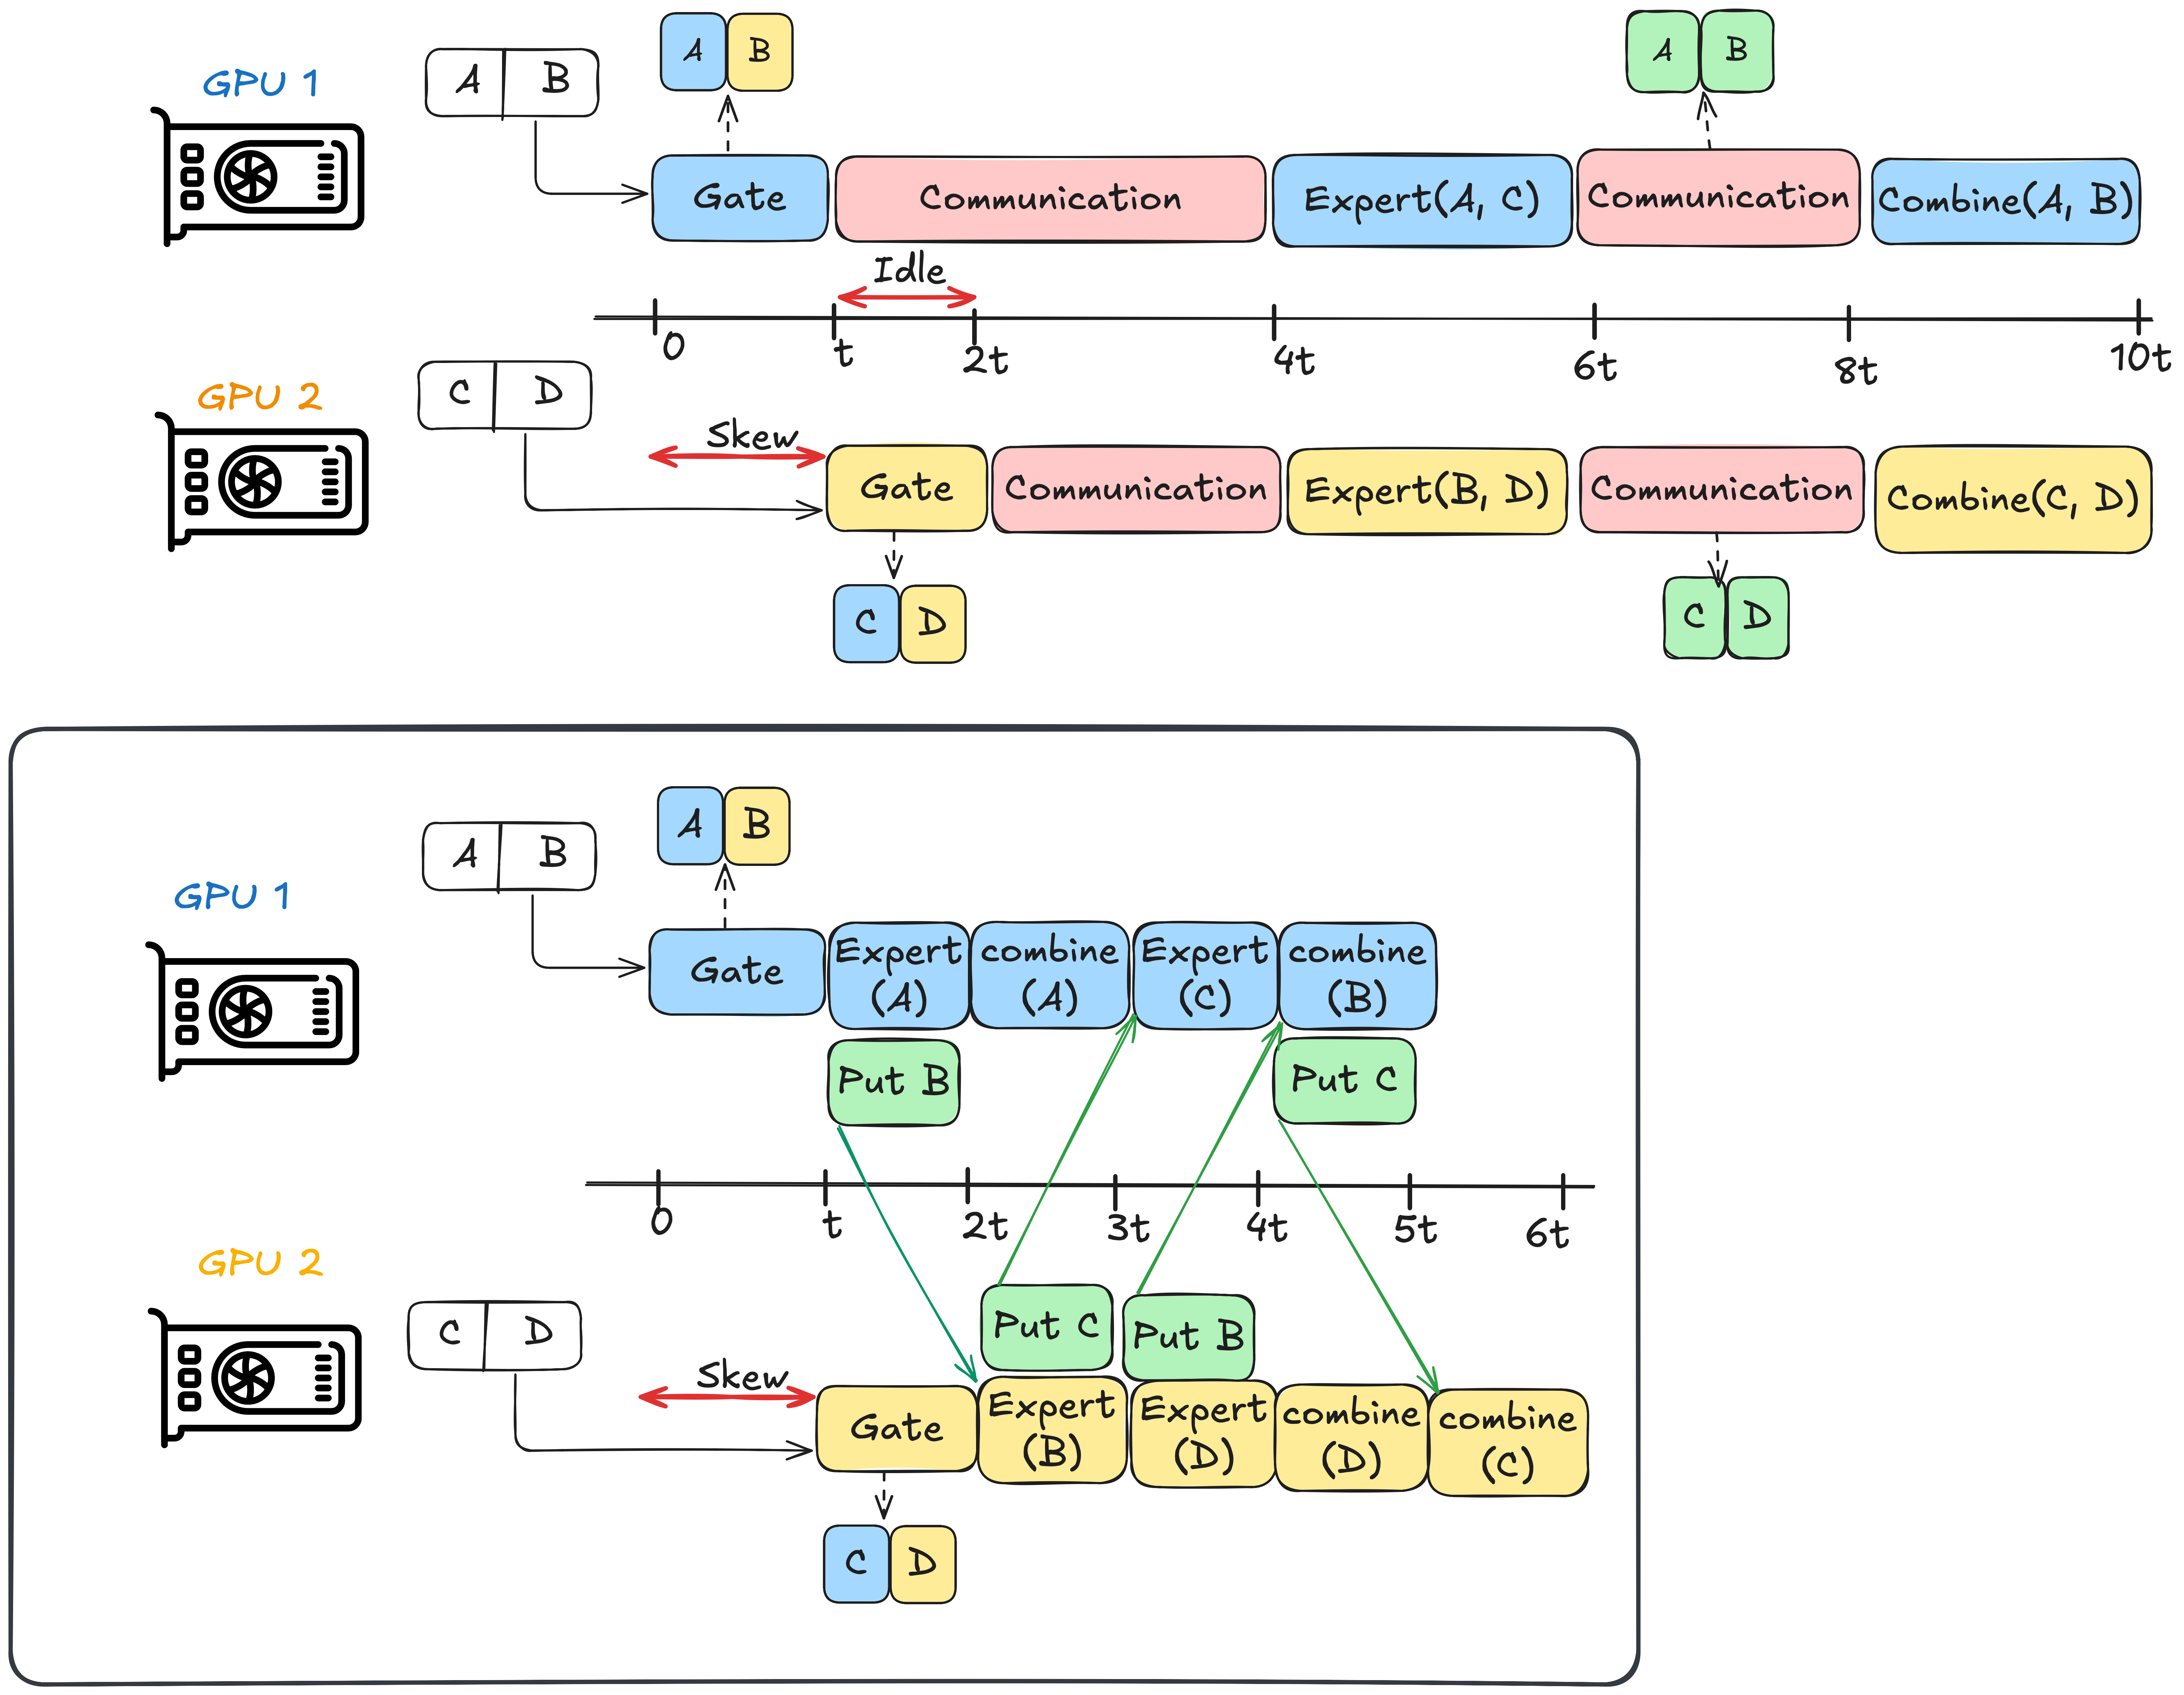
\includegraphics[width=0.8\textwidth, keepaspectratio]{figures/s_overlap}
    \caption{Overlapped Schedule (bottom) showing how idle time from the sequential schedule (top)
        is repurposed for computation. \sysname implements the overlapped schedule.}
    \label{fig:overlap}
\end{figure}
\alltoall communication as currently used in MoE frameworks is a ~\emph{synchronous} collective operation among
all participating GPUs. In this setting, disparities in processing speeds or kernel scheduling
among workers induce a straggler effect detrimental to the collective operation's performance.
Specifically, as shown in Figure~\ref{fig:straggler}, for distributed training of a 1.3B MoE model across 32 A100 GPUs,
we see P95 communication performance degradation of \textbf{1.32X} when compared to the mean actual kernel time
from Figure~\ref{sub:raw_perl}.
This performance reduction is rather tame as the underlying hardware is a supercomputer that is
well-tuned against ``software jitter''~\cite{nerscNetworkNERSC}.
The performance loss is more severe in a single node Virtual Machine (VM) of with higher bandwidth,
where we observe p95 performance reduction of \textbf{11X}.
In line with prior work~\cite{1639320, 10.1145/3545008.3545056} from the HPC community,
we argue that obviating the inherent barrier in this synchronous collective communication would
allow GPUs to repurpose this observed idle time for useful computation as depicted in Figure~\ref{fig:overlap}.
\subsection{Kernel launch overhead.}\label{subsec:kernel-launch-overhead.}
\begin{figure}[!h]
    \centering
    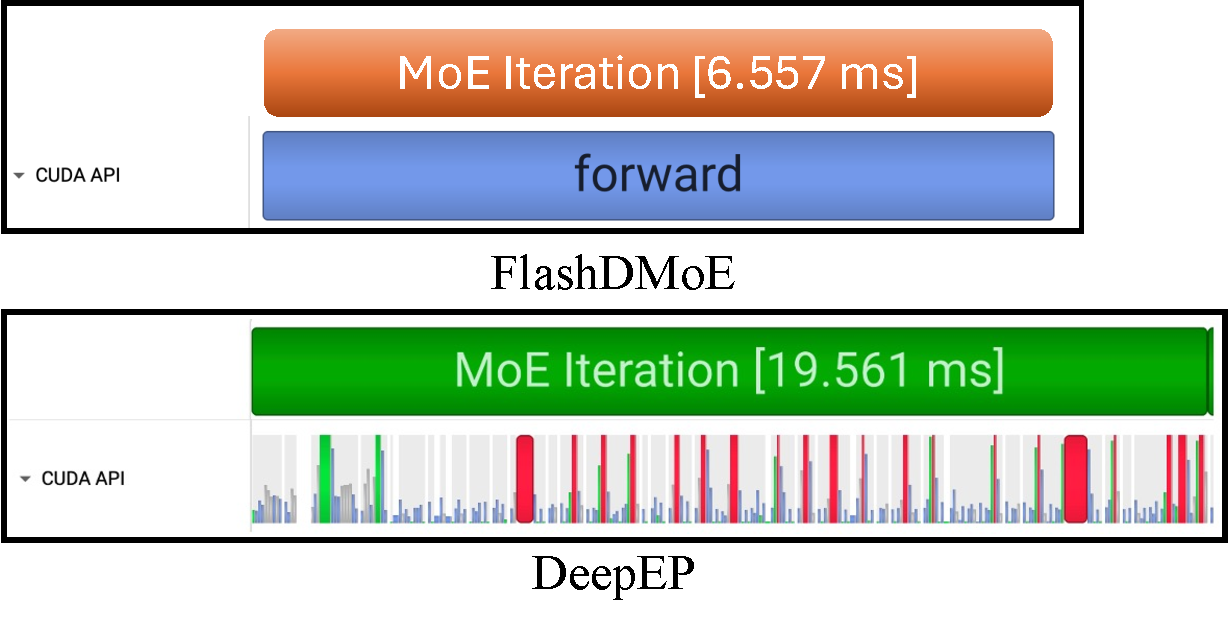
\includegraphics[width=0.6\textwidth, keepaspectratio]{figures/kernel_launch}
    \caption{Kernel Launch overhead (CUDA API row) juxtaposed with runtime latency.
    Compared to DeepEP that launches 432 kernels, \sysname launches a single one.}
    \label{fig:kl}
\end{figure}
We compare the kernel launch overheads between \sysname and existing baselines.
Table~\ref{tab:gpuOps} shows the number of kernel launches during a single forward pass: \sysname launches exactly one persistent kernel, while the baselines launch up to 550 short-lived kernels to perform the same computation.
Figure~\ref{fig:kl} provides a visual comparison using CUDA API traces captured by NSight Systems, illustrating the difference between \sysname and DeepEP.
DeepEP exhibits numerous small CUDA API calls, with frequent stalls between individual operators, leading to increased GPU idle time.
In contrast, \sysname maintains high GPU utilization by avoiding launch overhead and synchronization gaps—achieving 93.17\% GPU utilization compared to 20.61\% for DeepEP. See \S\ref{sec:evaluation} for experimental details and \S\ref{sec:related} for a discussion of related work.